%%%%%%%%%%%%%%%%%%%%%%%%%%%%%%%%%%%%%
%%%%%%%%%% Plantilla del Team para el proyecto final 
%%%%%%%%%%%%%%%%%%%%%%%%%%%%%%%%%%%%%
%%%%%%%%%% Nueva clase personalizada
\documentclass{staprojteamusb}
%%%%%%%%%% Nuevo estilo personalizado
\usepackage{staprojteamusbsty}

\addbibresource{referencias.bib}
%%%%%%%%%%%%%%%%%%%%%%%%%%%%%%%%%%%
%%%%%%%%%% Variables de Markdown
%%%%%%%%%%%%%%%%%%%%%%%%%%%%%%%%%%%
%%%%%%%%%% Encabezado 
\titulo{Análisis estadístico sobre jugadores la MLB.}

\autor{
		Miguel Cordero\\
	Universidad Simón Bolívar \\
	Caracas, Venezuela \\
	\texttt{\href{mailto:15-10326@usb.ve}{\nolinkurl{15-10326@usb.ve}}} \\
	 \And
		Eduardo Gavazut\\
	Universidad Simón Bolívar \\
	Caracas, Venezuela \\
	\texttt{\href{mailto:13-10524@usb.ve}{\nolinkurl{13-10524@usb.ve}}} \\
	 \And
		Luis Riera\\
	Universidad Simón Bolívar \\
	Caracas, Venezuela \\
	\texttt{\href{mailto:16-10976@usb.ve}{\nolinkurl{16-10976@usb.ve}}} \\
	}
\fecha{8 de abril de 2022}
\resumen{El deporte como actividad social del ser humano no es ajena a la ciencia, en particular, a la matemática y la estadística. En beisbol, por ejemplo, se recopila cada mínimo información de todo lo que sucede durante el juego, aspectos como: tasa de bateo, carreras anotadas o ponches. Y es que estos datos permiten medir cuan bueno o acertado es el desempeño de cada jugador. Debido a la gran cantidad de información, que además se ha incrementado con los años, es necesario recurrir a la ciencia y a modelos computacionales de predicción que ofrezcan un punto de objetividad que permita a los equipos mejorar su competitividad. En este trabajo, se mostrará como realizar un análisis estadítico sobre una base de datos de jugadores de la Major League Baseball (MLB), relativo a la tasa de bateo, carreras anotadas, triples, dobles y ponches por veces al bate. De este análisis se destaca el comprobar como la tasa de ponches es mayor a la tasa de jonrones de un jugador, y que es posible hallar una relación lineal entre las tasas de bateo y las tasas de carreras anotadas, de dobles y ponches por veces al bate. Esto permitirá predecir con un nivel 0.8589 de error cuadrático ajustado, cual será la tasa de carreras anotadas por jugador según su desempeño en el campo. Más aún, un análisis de varianza (ANOVA), permite demostrar que no hay mayor distinción entre entre jugadores con diferentes tasas de bateo.}

\palabrasc{Proyecto, Estadística, R, RStudio, Baseball, MLB, Predicción, ANOVA}
%%%%%%%%%%%% Resto de las variables propias de R eso viene por defecto de R

%%%%%%%% Pandoc Estilo  de los codigos
\usepackage{color}
\usepackage{fancyvrb}
\newcommand{\VerbBar}{|}
\newcommand{\VERB}{\Verb[commandchars=\\\{\}]}
\DefineVerbatimEnvironment{Highlighting}{Verbatim}{commandchars=\\\{\}}
% Add ',fontsize=\small' for more characters per line
\usepackage{framed}
\definecolor{shadecolor}{RGB}{248,248,248}
\newenvironment{Shaded}{\begin{snugshade}}{\end{snugshade}}
\newcommand{\AlertTok}[1]{\textcolor[rgb]{0.94,0.16,0.16}{#1}}
\newcommand{\AnnotationTok}[1]{\textcolor[rgb]{0.56,0.35,0.01}{\textbf{\textit{#1}}}}
\newcommand{\AttributeTok}[1]{\textcolor[rgb]{0.77,0.63,0.00}{#1}}
\newcommand{\BaseNTok}[1]{\textcolor[rgb]{0.00,0.00,0.81}{#1}}
\newcommand{\BuiltInTok}[1]{#1}
\newcommand{\CharTok}[1]{\textcolor[rgb]{0.31,0.60,0.02}{#1}}
\newcommand{\CommentTok}[1]{\textcolor[rgb]{0.56,0.35,0.01}{\textit{#1}}}
\newcommand{\CommentVarTok}[1]{\textcolor[rgb]{0.56,0.35,0.01}{\textbf{\textit{#1}}}}
\newcommand{\ConstantTok}[1]{\textcolor[rgb]{0.00,0.00,0.00}{#1}}
\newcommand{\ControlFlowTok}[1]{\textcolor[rgb]{0.13,0.29,0.53}{\textbf{#1}}}
\newcommand{\DataTypeTok}[1]{\textcolor[rgb]{0.13,0.29,0.53}{#1}}
\newcommand{\DecValTok}[1]{\textcolor[rgb]{0.00,0.00,0.81}{#1}}
\newcommand{\DocumentationTok}[1]{\textcolor[rgb]{0.56,0.35,0.01}{\textbf{\textit{#1}}}}
\newcommand{\ErrorTok}[1]{\textcolor[rgb]{0.64,0.00,0.00}{\textbf{#1}}}
\newcommand{\ExtensionTok}[1]{#1}
\newcommand{\FloatTok}[1]{\textcolor[rgb]{0.00,0.00,0.81}{#1}}
\newcommand{\FunctionTok}[1]{\textcolor[rgb]{0.00,0.00,0.00}{#1}}
\newcommand{\ImportTok}[1]{#1}
\newcommand{\InformationTok}[1]{\textcolor[rgb]{0.56,0.35,0.01}{\textbf{\textit{#1}}}}
\newcommand{\KeywordTok}[1]{\textcolor[rgb]{0.13,0.29,0.53}{\textbf{#1}}}
\newcommand{\NormalTok}[1]{#1}
\newcommand{\OperatorTok}[1]{\textcolor[rgb]{0.81,0.36,0.00}{\textbf{#1}}}
\newcommand{\OtherTok}[1]{\textcolor[rgb]{0.56,0.35,0.01}{#1}}
\newcommand{\PreprocessorTok}[1]{\textcolor[rgb]{0.56,0.35,0.01}{\textit{#1}}}
\newcommand{\RegionMarkerTok}[1]{#1}
\newcommand{\SpecialCharTok}[1]{\textcolor[rgb]{0.00,0.00,0.00}{#1}}
\newcommand{\SpecialStringTok}[1]{\textcolor[rgb]{0.31,0.60,0.02}{#1}}
\newcommand{\StringTok}[1]{\textcolor[rgb]{0.31,0.60,0.02}{#1}}
\newcommand{\VariableTok}[1]{\textcolor[rgb]{0.00,0.00,0.00}{#1}}
\newcommand{\VerbatimStringTok}[1]{\textcolor[rgb]{0.31,0.60,0.02}{#1}}
\newcommand{\WarningTok}[1]{\textcolor[rgb]{0.56,0.35,0.01}{\textbf{\textit{#1}}}}

%%%%%%%%% Estilo de las listas sin salto de linea
\providecommand{\tightlist}{%
	\setlength{\itemsep}{0pt}\setlength{\parskip}{0pt}}

%%%%%%%%%%  Estilo de las tablas propias de R
\usepackage{longtable,booktabs,array}
\usepackage{calc} % Para la minipaginas y sus tamaños
%%%%%%%%%% Para las tablas y los parrafos \paragraph o \subparagraph
\usepackage{etoolbox}
\makeatletter
\patchcmd\longtable{\par}{\if@noskipsec\mbox{}\fi\par}{}{}
\makeatother
% Para los pie de pagina en tablas largas
\IfFileExists{footnotehyper.sty}{\usepackage{footnotehyper}}{\usepackage{footnote}}
\makesavenoteenv{longtable}

%%%%%%%%%%%% Si hay paquetes por incluir en header-include
\usepackage{booktabs}
\usepackage{longtable}
\usepackage{array}
\usepackage{multirow}
\usepackage{wrapfig}
\usepackage{float}
\usepackage{colortbl}
\usepackage{pdflscape}
\usepackage{tabu}
\usepackage{threeparttable}
\usepackage{threeparttablex}
\usepackage[normalem]{ulem}
\usepackage{makecell}
\usepackage{xcolor}
%%%%%%%%%%%%%%%%%%%%%%%%%%%%%%%%%%%%%%%%%%%%%%%%%%%%%%%%%
\begin{document}
	
	
	\maketitle
	
	%%%%%%%%%%%% Si hay cosas que incluir en include-before
		%%%%%%%%%%%%%%%%%%%%%%%%%%%%%%%%%%%%%%%%%%%%%%%%%%%%%%%%%
	
	%%%%%%%%%%%%% Inicio del documento
	\vspace{-13mm}
	\hypertarget{planteamiento-del-problema}{%
 \subsection{Planteamiento del problema}\label{planteamiento-del-problema}}

 En el presente proyecto, el objetivo es tomar una base de datos (en este caso de diversas métricas que corresponden a jugadores de la MLB) y realizar distintos estudios sobre ella, los cuales serán:

 \begin{enumerate}
   \item Análisis descriptivo.
   \item Intervalo de confianza ($97\%$) para la media de cada variable.
   \item Probar (a nivel de 0.05) que el promedio de bateo es inferior a 0.300.
   \item Estudiar si la tasa de ponches y de jonrones son iguales.
   \item Prueba de bondad de ajuste para la tasa de bateo para determinar si tiene distribución normal.
   \item Gráfico de dispersión y matriz de correlación para las variables.
   \item Modelo de regresión lineal que prediga la tasa de bateo en función al resto de las variables.
   \item Separar a la tasa de bateo en tres grupos: los que tienen menos de 0.200, los que tienen entre 0.200 y 0.300, y los que tienen más de 0.300, y realización de un análisis de varianza para estudiar si los promedios de tasas de las otras variables son iguales.
 \end{enumerate}



 \hypertarget{descripciuxf3n-de-la-base-de-datos}{%
 \subsection{Descripción de la base de datos}\label{descripciuxf3n-de-la-base-de-datos}}

 La base de datos a estudiar cuenta con 45 observaciones de 6 variables, las cuales son:

 \begin{enumerate}
   \item X1 = tasa de bateo, calculada como hits/veces al bate. Entiéndase la conexión efectuada por el bateador que coloca la pelota dentro del terreno de juego, permitiéndole alcanzar al menos una base, sin que se produzca un error de defensa del equipo contrario o algún otro jugador sea declarado como fuera de juego.
   \item X2 = carreras anotadas/veces al bate. Entiéndase carrera por anotación, y se logra al recorrer un corredor la totalidad de las bases volviendo al home, bien de manera continua (por medio de un jonrón) o de forma alternada consecutiva antes de que se realicen 3 outs.
   \item X3 = dobles/veces al bate. Entiéndase por doble como un hit en el que el bateador logra llegar a segunda base sin ser puesto out y sin que haya error alguno de la defensiva. 
   \item X4 = triples/veces al bate. Entiéndase por triple como un hit en el que el bateador logra llegar satisfactoriamente a tercera base, sin que ocurra ningún error por parte de la defensiva.
   \item X5 = jonrones/veces al bate. Un jonrón se da cuando el bateador hace contacto con la pelota de una manera que le permita recorrer las bases y anotar una carrera (junto con todos los corredores en base) en la misma jugada, sin que se registre ningún out ni error de la defensa.
   \item X6 = ponches/veces al bate. Por último, un ponche es la acción de retirar a un bateador con una cuenta de 3 strikes, al que la recibe se le suele llamar ponchao o ponchado.
 \end{enumerate}

 De esta forma, vemos que cada una de las variables miden números bastante relevantes para cada jugador. Como cada una de estas estadísticas pueden ocurrir una sola vez mientras se está al bate, cada una será un numéro entre el 0 y el 1.

 \hypertarget{metododologuxeda}{%
 \subsection{Metododología}\label{metododologuxeda}}

 Para la realización de esta investigación se hará uso del sofware estadístico \texttt{R} en el entorno de desarrollo intergrado (IDE) \texttt{RStudio}. En este se iniciará por una descripción de los datos y variables almacenadas en el archivo fuente \emph{Baseball.xlsx}, tales como: mínimo, media, cuantiles y desviación estándar. Para la media de las variables se obtendrá un intervalo de confianza del \(95\%\). Como se desea estudiar la relación de la tasa de bateo respecto al resto de las variables, se buscará determinar la mejor distribución de probabilidad que se ajuste a esta variable. Finalmente, se estudiará la eficiencia del mejor modelo lineal de predicción que se ajuste a los datos y permita establecer si en efecto existe tal relación entre las variables y las implicaciones que tendría en las estrategias para futuros juegos de beisbol.

 \hypertarget{anuxe1lisis-de-los-datos}{%
 \subsection{Análisis de los datos}\label{anuxe1lisis-de-los-datos}}

 Para la realización de este proyecto se contó con una archivo de excel con la información de algunos jugadores de la Major League Beisbol o MLB, el cual se almacenó en una variable llamada \texttt{Baseball}. De esta archivo podemos realizar el siguiente análisis de datos.

 \hypertarget{quuxe9-clase-es-la-base-de-datos}{%
 \subsubsection{¿Qué clase es la base de datos?}\label{quuxe9-clase-es-la-base-de-datos}}

 Con el comando \texttt{class}, se pudo determinar el tipo de base de datos utilizada o lo que es equivalente, la clase de la variable \texttt{Baseball}. El resultado que se obtuvo indica que es del tipo \texttt{tbl\_df}, que es una subclase de la clase \texttt{data.frame}. \texttt{tbl\_df} cumple con tener propiedades diferentes por defecto y se suele referir a ellas como \texttt{tibble}. Es una clase eficiente para trabajar con bases de datos grandes y su visualización.

 \hypertarget{variables-en-la-base-de-datos}{%
 \subsubsection{Variables en la base de datos}\label{variables-en-la-base-de-datos}}

 Si se desea saber que tipo de variables están almacenadas en la base de datos, se puede utilizar el comando \texttt{str}. Esta función nos indica que se cuentan con \(6\) variables denominadas \texttt{X1,X2,X3,X4,X5,X6}, y distribuidas de tal manera que representan la columnas de la base de datos. Cada una de estas variables tienen \(45\) valores de tipo \texttt{double} o número decimal, que representan las \(45\) observaciones aleatorias (una por fila) realizadas a jugadores de la (MLB).

 \hypertarget{estaduxedsticos}{%
 \subsubsection{Estadísticos}\label{estaduxedsticos}}

 Para obtener los estadísticos de las seis (6) variables de esta base de datos, se inicia por guardar las \(45\) observaciones en un vector que represente a cada variable.

 Con los datos vectorizados se pueden aplicar las siguientes funciones: \texttt{mean} que permite obtener la media de los datos, \texttt{median} para obtener la mediana, \texttt{quantile} para retornar los cuantiles al \(0.25\%, 0.50\%\) y \(0.75\%\) de cada variable, \texttt{min} para el valor mínimo, \texttt{max} para el valor máximo, \texttt{var} para la varianza, \texttt{sd} que es para la desviación estándar, \texttt{IQR} es para el rango intercuartil y finalmente, el coeficiente de variación obtenido como \texttt{stad/media}.

 \begin{table}[h]
 \centering
 \resizebox{\linewidth}{!}{
 \begin{tabular}[t]{l|c|c|c|c|c|c|c|c|c|c}
 \hline
   & Mínimo & 25\% & Media & Mediana (50\%) & 75\% & Máximo & RIC & Varianza & Desv. Estándar & Coef. Variación\\
 \hline
 X1 & 0.188 & 0.248 & 0.2805 & 0.290 & 0.308 & 0.367 & 0.060 & 0.0019 & 0.0440 & 0.1569\\
 \hline
 X2 & 0.064 & 0.119 & 0.1509 & 0.150 & 0.189 & 0.259 & 0.070 & 0.0018 & 0.0420 & 0.2784\\
 \hline
 X3 & 0.025 & 0.039 & 0.0464 & 0.045 & 0.053 & 0.068 & 0.014 & 0.0001 & 0.0105 & 0.2255\\
 \hline
 X4 & 0.001 & 0.007 & 0.0113 & 0.009 & 0.016 & 0.030 & 0.009 & 0.0000 & 0.0070 & 0.6165\\
 \hline
 X5 & 0.000 & 0.009 & 0.0243 & 0.013 & 0.039 & 0.085 & 0.030 & 0.0005 & 0.0223 & 0.9173\\
 \hline
 X6 & 0.000 & 0.062 & 0.1043 & 0.095 & 0.138 & 0.264 & 0.076 & 0.0040 & 0.0631 & 0.6044\\
 \hline
 \end{tabular}}
 \caption{\label{tab:resumen}Resumen Estadístico de las variables}
 \end{table}

 Los resultados pueden ser apreciados en la tabla \ref{tab:resumen}. De estos resultados hay varios puntos que podemos detacar. La varianza de los datos es muy baja indicativo que entre los datos hay pocos valores atípicos o muy dispersos, lo que se refleja en valores mas cercanos a la media. Misma interpretación se puede extender a la desviación estándar pues es la raíz cuadrada de la varianza.

 Una consecuencia de la baja varianza es que la media y la mediana son valores muy cercanos. Esto es particularmente útil al analizar el valor del \texttt{RIC}, que toma como medida central la mediana de los datos. Es decir, nos indica donde se encuentra el \(50\%\) de los datos, cuánto mas bajo es el valor del RIC menos dispersos están los datos.

 \hypertarget{diagramas-e-histograma-de-los-datos-por-cada-variable}{%
 \subsubsection{Diagramas e histograma de los datos por cada variable}\label{diagramas-e-histograma-de-los-datos-por-cada-variable}}

 De la figura \ref{fig:boxplots}, podemos establecer: para la variable \texttt{X1}, que los valores máximos de los datos se obtienen luego de la media, pero el mayor volumen de ellos se encuentra antes como bien se observa en el diagrama de caja que permite confirmar, además, la ausencia de datos atípicos. Para la variable \texttt{X2}, se puede comprobar que ver simetría de los datos que se infería de la tabla \ref{tab:resumen}, particularmente respecto al valor \(0.15\) que coincide a su vez con la media de los datos. El diagrama de caja permite confirmar la ausencia de los valores atípicos.

 Por su parte, para la variable \texttt{X3} y \texttt{X4}, Vemos que en general, ambos diagramas de caja son bastante parecidos, con la única diferencia siendo que el de triples está \(0.03\) puntos corrido hacia arriba y los datos desde el primer cuartil hasta la mediana están muchos más dispersos. Otra diferencia es que el diagrama de cajas para los triples no cuenta con datos atípicos, en cambio los dobles si, que corresponde a \(0.3\). Todo esto hace que el diagrama de los triples sea casi simétrico, y el de los dobles sea más chato entre el valor mínimo y la mediana, en comparación con lo que tenemos entre la mediana y el máximo valor.

 De la gráfica para la variable \texttt{X5} podemos ver como a medida que nos vamos acercando a \(1\), la frecuencia de jonrones decae rapidamente, mientras que al incio es muy alta. De la gráfica para la variable \texttt{X6} podemos ver que la mayoría de los jugadores se ponchan menos de un \(15\%\) de las veces que estan al bate.

 \hypertarget{intervalo-de-confianza-para-la-media-de-las-variables}{%
 \subsection{Intervalo de confianza para la media de las variables}\label{intervalo-de-confianza-para-la-media-de-las-variables}}

 Con el uso de la función \texttt{t.test()} se puede encontrar el intervalo de confianza con una significancia de \(0.03\) o \(97\%\) de confianza para las variables estudiadas. Los resultados de aplicar esta función, se pueden visualizar en la tabla \ref{tab:intervals}.

 \begin{table}[h]

 
 \centering
 \begin{tabular}[t]{l|l|c|c}
 \hline
   & Limite inferior & Promedio & Limite Superior\\
 \hline
 Tasa de bateo & 0.2658 & 0.2805 & 0.2952\\
 \hline
 Carreras anotadas & 0.1368 & 0.1509 & 0.1649\\
 \hline
 Dobles & 0.0429 & 0.0464 & 0.0498\\
 \hline
 Triples & 0.0090 & 0.0113 & 0.0136\\
 \hline
 Jonrones & 0.0168 & 0.0243 & 0.0317\\
 \hline
 Ponches & 0.0833 & 0.1043 & 0.1254\\
 \hline
 \end{tabular}
 \caption{\label{tab:intervals}Intervalos de confianza para las medias de las variables}
 \end{table}

 Se pueden visualizar mejor estos intervalos de confianza, en la figura \ref{fig:interconf} de los anexos.

 Note que en general, los intervalos de confianza más estrechos son los de dobles y triples, lo que nos indica que en general, con una probabilidad del \(97\%\), podemos asegurar que los jugadores de la MLB tendrán un promedio de triples y dobles que puede ser estimado con bastante certeza, pero vemos que las carreras anotadas, los ponches y la tasa de bateo tienen un intervalo de confianza mucho más grande, por lo que no podemos asegurar que el promedio será estimado de forma tan certera.

 \hypertarget{promedio-de-bateo}{%
 \subsection{Promedio de bateo}\label{promedio-de-bateo}}

 Con lo obtenido en los intervalos de confianza del apartado anterior se tiene que la tasa de bateo toma valores por debajo de \(0.300\). Para corroborar este resultado, se realizará un prueba de hipótesis con un nivel de significancia de \(\alpha=0.05\).

 Entonces, como hipótesis nula \(H_{0}\) y como hipótesis altenativa \(H_{a}\) tenemos: vamos a suponer que la media de bateo, \(H_{0}: \mu_{\operatorname{bateo}}\leq 0.3,\qquad H_{\alpha}: \mu_{\operatorname{bateo}}> 0.3\)

 Si suponemos que los datos presentan una distribución normal, podemos aplicar el comando \texttt{t.test} de \texttt{R}, que permite realizar pruebas de hipótesis sobre las medias de los datos cuando se trabaja con una sola variable.

 Con esta función, se obtuvo que el valor para el estadístico \(t\) es \(-23.811\), con \(44\) grados libertad. Como el \(p-valor\) es bastante alto, de hecho es igual \(0,9976\) (que representa un \(99.76\%\)), se cumple que \(\alpha=0.05<99.76\) y por lo tanto la hipótesis alternativa se rechaza, mas aún, se rechaza para todo nivel de significancia porque se necesita un valor para \(\alpha\) más alto que el \(p-valor\) para rechazar la hipótesis nula.

 Se afirma entonces, con total seguridad, que la tasa de bateo es inferior a \(0.300\), tal como se podía con el intervalo de confianza.

 \hypertarget{comparaciuxf3n-entre-las-tasas-de-ponches-y-las-de-jonrones}{%
 \subsection{Comparación entre las tasas de ponches y las de jonrones}\label{comparaciuxf3n-entre-las-tasas-de-ponches-y-las-de-jonrones}}

 Ahora, deseamos comparar las tasas de ponches y de jonrones para determinar si o no parecidas. Como no tenemos conocimiento acerca de las varianzas poblacionales, usaremos el test de Welch tal y como es explicado en Heumann, Schomaker (2017) para comparar las medias. En este caso, haremos una prueba de hipótesis, donde tomaremos como hipótesis nula, \(H_{0}\) e hipótesis alternativa \(H_{a}\) las dadas por: \linebreak 
 \(H_0 : \mu_{\operatorname{jonrones}} - \mu_{\operatorname{ponches}} = 0 \quad \text{ vs. } \quad H_a : \mu_{\operatorname{jonrones}} - \mu_{\operatorname{ponches}} \neq 0\)

 Es decir, queremos determinar si las tasas de jonrones y ponches son distintas. Ahora, con apoyo del comando anterior \texttt{t.test()}, pero esta vez para comparar dos variables, podremos determinar cuál de estas hipótesis es aceptada.

 Como resultado se obtuvo que el \(\operatorname{p-valor}=1.112\times 10^{-8}\), que es extremadamente pequeño, mucho más que el nivel de significancia \(\alpha = 0.01\) que es razonable utilizar para nuestra prueba de hipótesis. Adicionalmente, el intervalo de confianza que se obtuvo fue de \((-0.1068,-0.0593)\) que no incluye el cero. Otra cosa que podemos hacer es evaluar el estadístico de prueba con el comando \texttt{qt()} (vemos por lo anterior que \(dt = 55\) y \(\alpha = 0.05\)).

 Como \(t=-8\), vemos que el estadístico cae en la región de rechazo (porque es de cola doble).

 Para cualquiera de estos casos, podemos concluir que la hipótesis nula se rechaza, es decir que hay suficiente evidencia para creer que \(\mu_{\operatorname{jonrones}} - \mu_{\operatorname{ponches}} \neq 0\). Y además, como el intervalo de confianza es negativo, concluimos que \(\mu_{\operatorname{ponches}} > \mu_{\operatorname{jonrones}}\) con un nivel de confianza del \(95\%\), como se podía apreciar de la figura \ref{fig:interconf}

 \hypertarget{prueba-de-bondad-de-ajuste-para-la-distribuciuxf3n-de-x1}{%
 \subsection{Prueba de bondad de ajuste para la distribución de X1}\label{prueba-de-bondad-de-ajuste-para-la-distribuciuxf3n-de-x1}}

 \begin{figure}[h]
 \centering
 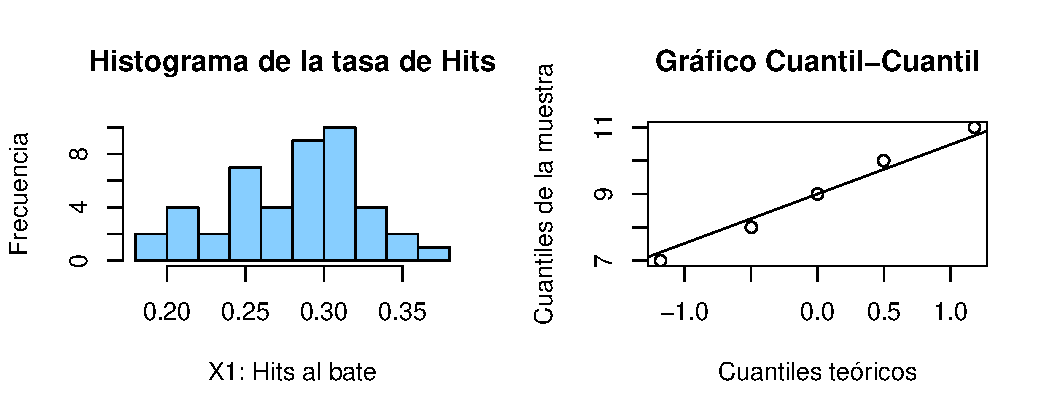
\includegraphics{C03322-InformeFinal-Cordero-Gavazut-Riera_files/figure-latex/cuantilcuantil-1.pdf}
 \caption{\label{fig:cuantilcuantil}Histograma y Gráfico cuantil-cuantil de la variable X1}
 \end{figure}

 Para continuar con el análisis a un nivel más profundo, resulta conveniente determinar si los datos en la variable \texttt{X1}, sobre la tasa de bateos, sigue una distribución normal.

 Como se señaló en la figura \ref{fig:boxplots}, del histograma para la variable, obtenemos entonces que si subdividimos en intervalos de longitud \(0.02\) , las frecuencias son como las descritas en la tabla \ref{tab:tablafrecuencias}.

 \begin{table}[h!]
 \begin{tabular}{lccclcccccll}
 \hline
 \textit{\textbf{Intervalo}} & 0,18- 0,20 &  & 0,22- 0,24 &  & 0,26- 0,28 &  & 0,30-0,32 &  & 0,34-0,36 &  & \multicolumn{1}{c}{0,38} \\ \hline
 \textit{\textbf{Frecuencia}} & 2 & 4 & 2 & \multicolumn{1}{c}{4} & 7 & 9 & 10 & 4 & 2 & \multicolumn{1}{c}{1} &  \\ \hline
 \end{tabular}
 \caption{\label{tab:tablafrecuencias}Tabla de clases y frecuencias}
 \end{table}

 Ahora agruparemos los datos en categorías de frecuencia mayor o igual a 5 (para poder aplicar el método de bondad de ajuste) tal como puede apreciarse en la tabla \ref{tab:nuevasClases}.

 \begin{table}[h]
 \begin{tabular}{lccccc}
 \hline
 \textit{\textbf{Clases}} & [0,18 \quad  0,24) &  [0,24 \quad 0,28) &  [0.28\quad 0,30) & [0.30\quad 0,32) & [0.32\quad  0,38) \\ \hline
 \textit{\textbf{Frecuencia}} & 8  & 11 & 9 & 10 & 7  \\ \hline
 \end{tabular}
 \caption{\label{tab:nuevasClases}Nueva agrupación en clases con frecuencia mayor o igual a 5}
 \end{table}

 Con la gráfica cuantil-cuantil de la figura \ref{fig:cuantilcuantil}, podemos ver que esta agrupación se ajusta bien a un distribución normal (representada por la recta).
 

 Vamos a proceder a realizar una prueba \(\chi^{2}\), que es una prueba de hipótesis que compara la distribución observada de los datos con la distribución esperada de los datos. Para este tipo de pruebas, el estadístico de \(\chi^{2}\) cuantífica que tanto varía la distribución respecto a la distribución hipotética. La hipótesis nula \(H_{0}\) y la hipótesis altenativa \(H_{a}\) vienen dadas por:
 \(H_{0}: \mbox{Los datos siguen una distribución normal}\) \(H_{a}: \mbox{Los datos no siguen una distribución normal}\)

 Como estadístico \(\chi^{2}\) tenemos: \(\displaystyle X^{2}=\sum_{i=1}^{k}\frac{[n_{i}-E(n_{i})]^{2}}{E(n_{i})}\)
 con \(k=5\) el número de clases o categorías, \(n_{i}\) las frecuencias de cada categoría, \(E(n_{i})=n*p_{i}\) el valor esparado con \(n\) el número total de datos y \(p_{i}\) la probabilidad de cada clase \(n_{i}\).

 Para calcular las probabilidades \(p_{i}\) se obtuvo la media y la desviación estándar de los datos agrupados como \(\bar{x}=0.2822\) y \(\sigma=0.045\), respectivamente. Con \(\bar{x}\) y \(\sigma\) se obtuvieron las siguientes probabilidades para cada clase: \(p_{1}=0.172,\ p_{2}=0.3082,\ p_{3}= 0.1747,\ p_{4}= 0.1466,\ p_{5}= 0.1986\).

 Sustituyendo los datos en el estadístico tenemos que: \(\chi^{2}=2.9421\), y el \(p-valor\) viende dado por \(1-P(\chi^{2}<2.9421)=0.2297\). El \(p-valor\) es bastante alto por lo que la hipótesis nula no se rechaza para ningún nivel de significancia. Por tanto los datos siguen una distribución normal con media \(0.2822\) y deviación estándar \(0.045\).

 \hypertarget{gruxe1fico-de-dispersiuxf3n-y-matrix-de-correlaciuxf3n}{%
 \subsection{Gráfico de dispersión y matrix de correlación}\label{gruxe1fico-de-dispersiuxf3n-y-matrix-de-correlaciuxf3n}}

 Es ahora, de nuestro interés estudiar la relación entre las variables de la base de datos. Esto lo podemos observar en la figura \ref{fig:correlacion}. Note que las gráficas de dispersión de la mitad inferior de la figura \ref{fig:correlacion}, se puede apreciar que para carreras anotadas, dobles y triples tenemos algo que se asemeja a una relación lineal positiva, mientras que para los ponches, estos disminuyen a medida que la tasa de bateo aumenta. La única variable que no parece tener ninguna relación clara con la tasa de bateo es la tasa de jonrones, por lo que es una variable que probablemente no nos ofrezca mayor información si queremos establecer un modelo lineal que relacione a las variables.

 Por otro lado, con la parte superior de la figura \ref{fig:correlacion} se tienen los coeficientes de correlación por pares de variables. Estos coeficientes nos indican que, efectivamente, para las carreras, dobles y triples, tenemos una correlación positiva (siendo las carreras la que tiene mayor correlación, y los triples la menor). Además, para los ponches tenemos una correlación negativa bastante significativa, y entre todas las variables, los jonrones tienen la menor correlación.

 \begin{figure}[h]
 \centering
 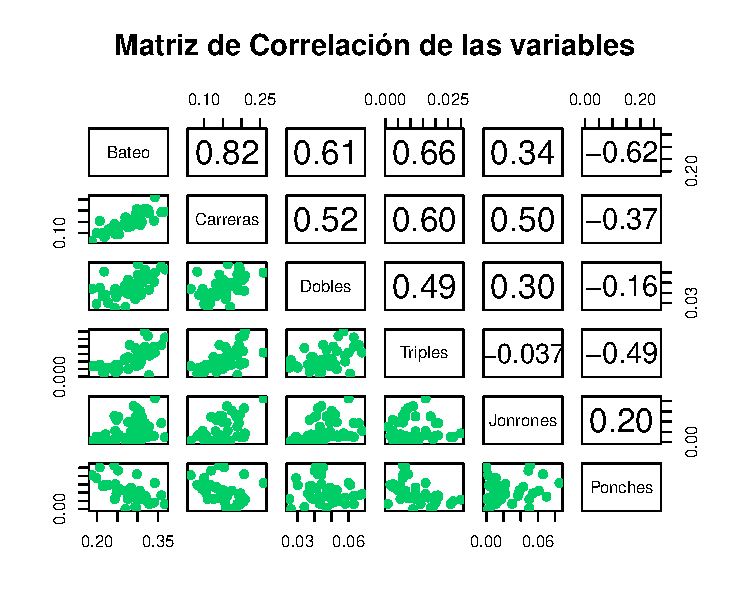
\includegraphics{C03322-InformeFinal-Cordero-Gavazut-Riera_files/figure-latex/correlacion-1.pdf}
 \caption{\label{fig:correlacion}Matrix de correlación y dispersión de las variables}
 \end{figure}

 \hypertarget{muestreo-80-20}{%
 \subsection{Muestreo 80\%-20\%}\label{muestreo-80-20}}

 Como por la figura \ref{fig:correlacion}, parece existir una relación lineal entre las variables, particularmente vamos a estar interesados en ver como se relaciona cada campo información (carreras, dobles, etc.) con la variable \texttt{X1} que es la tasa de bateo. Con \texttt{R} tenemos la posibilidad de obtener un modelo de regresión lineal con la función \texttt{lm}.

 Pero para asegurarnos que el modelo sea el más adecuado, primero necesitamos extraer una muestra que permita que entrenar al modelo de predicción, y con los datos restantes probar que tan eficiente es el modelo. Con este objetivo, se dividen los datos en un \(80\%\) para el entrenamiento y en un \(20\%\) para las pruebas.

 Como la base base de datos consta de \(45\) observaciones por variable, el \(80\%\) representa tomar una muestra aleatoria de \(36\) observaciones, por los que el \(20\%\) restante serán las \(9\) no tomadas en la muestra. Vale la pena resaltar que se habla de observaciones, o las filas de la base de datos y no de las entradas particulares de cada variable porque se busca estudiar la relación por jugador, de su tasa de bateo, respecto a su tasa de carreras, dobles, triples, jonrones y ponches. En otras palabras, las filas son independientes entre sí y por eso se pueden tomar muestras al azar, pero las columnas no lo son por ser datos relativos a un jugador en particular.

 \hypertarget{modelo-de-regresiuxf3n-lineal-para-la-variable-x1}{%
 \subsection{Modelo de regresión lineal para la variable X1}\label{modelo-de-regresiuxf3n-lineal-para-la-variable-x1}}

 Ahora, teniendo seleccionado nuestros datos, podemos pasar a realizar el modelo.

 La mejor manera de realizar un modelo de regresión lineal es seguir el método de \textbf{regresión paso a paso}, de esta manera determinar cuáles variables son significativas o no al tomar en cuenta la tasa de bateo.

 Ahora, pasemos a realizar el modelo lineal utilizando el comando \texttt{lm()} de R. Se desarrolla primero el modelo dado por \(Y=\beta_{0}+\beta_{1}x_{1}+\beta_{2}x_{2}+\beta_{3}x_{3}+\beta_{4}x_{4}+\beta_{5}x_{5}+\epsilon\). Suponiendo que \linebreak \(E(\epsilon)=0\), buscamos estimar los parámetro \(\beta_{i}\) para los cuales \(E[Y]=\beta_{0}+\beta_{1}x_{1}+\beta_{2}x_{2}+\beta_{3}x_{3}+\beta_{4}x_{4}+\beta_{5}x_{5}\).

 Con el comando \texttt{lm()} se obtuvo que el único valor no significativo (y de hecho el p-valor más alto) fue la tasa de triples, seguido de la tasa de jonrones que era significativa a nivel \(0.05\).

 De esta forma, realicemos de nuevo el modelo pero sin la variable \(X4\) correspondiente a los triples. Es decir, el modelo a estimar es: \(E[Y]=\beta_{0}+\beta_{1}x_{1}+\beta_{2}x_{2}+\beta_{4}x_{4}+\beta_{5}x_{5}\).

 Con \texttt{R} se obtuvo en esta prueba, que la tasa de jonrones es la variables con p-valor mas alto, con \(0.0611\). A pesar, de ser significativa a nivel de \(0.1\) procedemos a realizar una nueva prueba, esta vez sin la tasa de jonrones.

 El nuevo modelo, consiste en estimar \(E[Y]=\beta_{0}+\beta_{1}x_{1}+\beta_{2}x_{2}+\beta_{5}x_{5}\). Ahora, todas nuestras variables son bastante significativas, por lo que sus p-valores son bastante pequeños, significativos a nivel \(0.001\). Los valores estimados fueron: \(\beta_{0}=0.1630\), \(\beta_{1}=0.5192\), \(\beta_{2}=1.3650\) y \(\beta_{6}=-0.2451\).

 Como medida del error, tenemos el \(R^{2}_{ajus}\), con valor \(0.8489\), indicando que hay un buen ajuste de los datos al modelo.

 Además, tenemos que:

 \begin{enumerate}
   \item Para los estimadores, los dobles es el mayor de todos, y este nos indica que por cada aumento del $1\%$ en la tasa de dobles, hay un aumento correlacionado del $136\%$ en la tasa de bateo. Es interesante ver que este estimador es muchísimo mayor que el de las carreras.
   \item La varianza es estimada como $\hat{\sigma}^2 = 0.01705^2$.
   \item Para el error estándar (Std. Error), podemos construir los intervalos de confianza para las variables. Primero, tenemos que $t_{32, 0.975} = 2.0369$: $I_{carreras} = 0.5192 \pm 2.0369*0.0868 = (0.3424, 0.6960)$. \linebreak $I_{dobles} = 1.3650 \pm 2.0369*0.3471 = (0.6580, 2.0720)$ $;\quad I_{ponches} = -0.2451 \pm 2.0369*0.0460 = (-0.3388, -0.1514)$
   
 Como ninguno de estos intervalos incluye el $0$, se puede concluir que efectivamente hay una relación existente entre estas variables seleccionadas y la tasa de bateo.
 \end{enumerate}

 Ahora, veamos que efectivamente se cumple con las característica de un buen modelo apoyándonos en las gráficas de la figura \ref{fig:modelo}.

 \begin{figure}
 \centering
 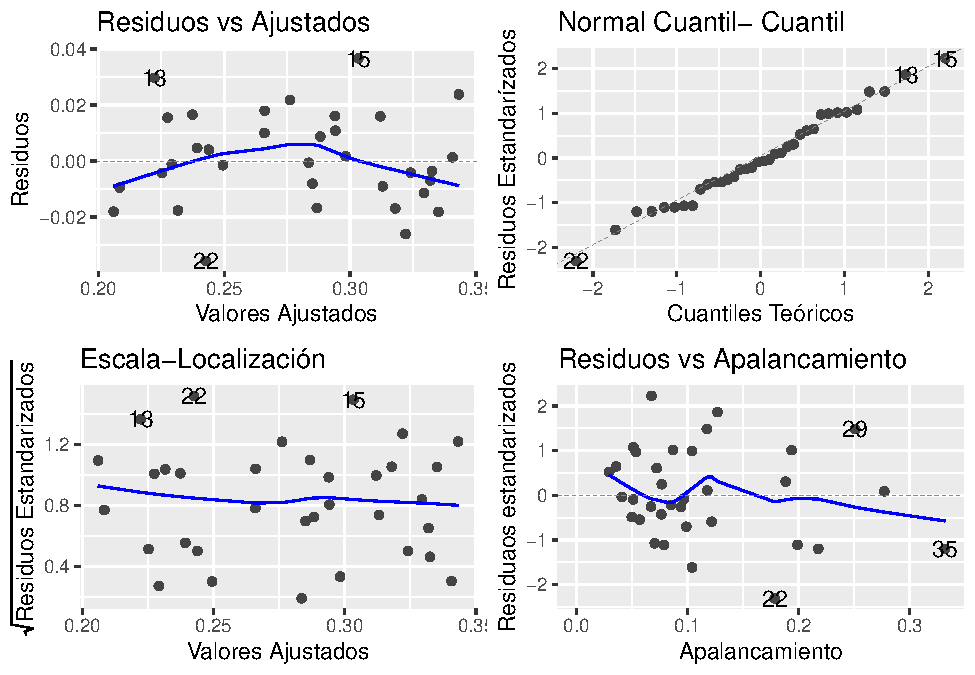
\includegraphics{C03322-InformeFinal-Cordero-Gavazut-Riera_files/figure-latex/modelo-1.pdf}
 \caption{\label{fig:modelo}Graficos descriptivos del modelo}
 \end{figure}

 \begin{itemize}
   \item Cuando vemos la gráfica de $``$Residuos vs Ajustados$"$, nos damos cuenta de que la línea roja es bastante horizontal, y esta además está centrada alrededor del cero, es decir que podemos asumir que no hay independencia entre las variables y la tasa de bateo.
   \item Al ver el gráfico "Normal Cuantil-Cuantil", vemos que todos los valores están bastante cercanos a la recta, lo que nos confirma la normalidad.
   \item En $``$Escala-Localización$"$ no vemos ningún patrón, lo que nos indica que los valores presentan homocedasticidad.
   \item Y por último, en $``$Residuos vs Apalancamiento$"$, no hay ningún valor que esté fuera de las líneas rayadas, por lo que no parece haber valores que generen apalancamiento.
 \end{itemize}

 En conclusión, podemos ver que este es un buen modelo, cuyas variables son todas significativas, no tiene datos que generen apalancamiento y cumple con homocedasticidad.

 Sintetizando, nuestro modelos es:
 \(\hat{Y}=0.1630+(0.5192)x_2+(1.3605)x_3-(0.2451)x_5\)

 \hypertarget{prueba-y-predicciuxf3n-del-modelo-lineal}{%
 \subsection{Prueba y predicción del modelo lineal}\label{prueba-y-predicciuxf3n-del-modelo-lineal}}

 Ahora, haremos uso del comando \texttt{predict} para hacer la predicción de la variable X1 (tasa de hits), utilizando las \(9\) observaciones que se seleccionaron previamente.

 Luego calculamos la diferencia entre los valores reales y los valores estimados por el modelo. Los resultados se muestran en la tabla \ref{tab:prediccion}. Es claro que los residuos son bastante pequeños, así que se considera que el modelo es suficientemente bueno para predecir la tasa de hits.

 \begin{table}[h]

 \caption{\label{tab:prediccion}Hits reales vs Hits predichos}
 \centering
 \begin{tabular}[t]{c|c|c}
 \hline
 Tasa de hits real  &  Tasa de hits predicha  &  Diferencia \\
 \hline
 0.281 & 0.2817371 & -0.0007371\\
 \hline
 0.290 & 0.2638287 & 0.0261713\\
 \hline
 0.269 & 0.3130776 & -0.0440776\\
 \hline
 0.307 & 0.3310601 & -0.0240601\\
 \hline
 0.308 & 0.2455406 & 0.0624594\\
 \hline
 0.358 & 0.2242784 & 0.1337216\\
 \hline
 0.245 & 0.3030698 & -0.0580698\\
 \hline
 0.294 & 0.2396552 & 0.0543448\\
 \hline
 0.218 & 0.2968785 & -0.0788785\\
 \hline
 \end{tabular}
 \end{table}

 \hypertarget{anova-para-la-tasa-de-bateo}{%
 \subsection{ANOVA para la Tasa de Bateo}\label{anova-para-la-tasa-de-bateo}}

 Para finalizar, estamos interesados en realizar un análisis de varianza sobre la variable \texttt{X1} O la tasa de bateo, para compararla con el resto de los variables. Particularmente queremos realizar, el estudio sobre \(3\) categorías o grupos:

 \begin{itemize}
 \tightlist
 \item
   Grupo 1: los bateadores con una tasa de bateo igual a \((X1<0.200)\).
 \item
   Grupo 2: los bateadores con una tasa de bateo igual a \((0.200\leq X1 < 0.300)\).
 \item
   Grupo 3: los bateadores con una tasa de bateo igual a \((0.300\leq X1)\)
 \end{itemize}

 Con esta agrupación se opta por realizar un análisis de varianza con bloques aleatorizados, donde los bloques serán los grupos y los tratamientos o métodos serán las distintas variables de la base de datos.

 Con la tabla \ref{tab:preANOVA} podemos apreciar las medias de los valores agrupados. Con estos valores, se puede aplicar el comando \texttt{anova} de \texttt{R} para obtener la tabla ANDEVA, tal y como se detalla en la tabla \ref{tab:andeva}.

 En esta tabla, se aprecia que el p-valor para lo grupos es de \(0.6198\) que es alto, indicando que la hipótesis nula para los grupos no se puede rechazar, es decir, que las medias por grupos son iguales. Sin embargo, para las medias clasificadas por variable o método se obtuvo un p-valor de \(0.0004\) que es bastante bajo, incluso significativo indicando que las medias son distintas tal como se esperaba por los datos analizados.

 Con esto podemos afirmar con seguridad, que los promedios de las tasas son iguales por cada grupo.

 \begin{table}[h]

 \caption{\label{tab:preANOVA}Tabla a dos factores para las medias de las variables}
 \centering
 \begin{tabular}[t]{l|r|r|r|r|r|r}
 \hline
   & X1 & X2 & X3 & X4 & X5 & X6\\
 \hline
 Grupo1 & 0.1935000 & 0.0820000 & 0.0365000 & 0.0070000 & 0.00650 & 0.1965000\\
 \hline
 Grupo2 & 0.2580400 & 0.1327600 & 0.0414400 & 0.0087200 & 0.02228 & 0.1204800\\
 \hline
 Grupo3 & 0.3212778 & 0.1837222 & 0.0542778 & 0.0153333 & 0.02900 & 0.0716667\\
 \hline
 \end{tabular}
 \end{table}

 \begin{table}[h]

 \caption{\label{tab:andeva}Tabla ANDEVA}
 \centering
 \begin{tabular}[t]{l|r|r|r|r|r}
 \hline
   & Df & Sum Sq & Mean Sq & F value & Pr(>F)\\
 \hline
 grupos & 2 & 0.0019826 & 0.0009913 & 0.5020692 & 0.6197546\\
 \hline
 variables & 5 & 0.1334024 & 0.0266805 & 13.5132135 & 0.0003524\\
 \hline
 Residuals & 10 & 0.0197440 & 0.0019744 & NA & NA\\
 \hline
 \end{tabular}
 \end{table}

 \hypertarget{conclusiones}{%
 \subsection{Conclusiones}\label{conclusiones}}

 De todo el análisis anterior se deduce que:

 \begin{enumerate}
 \def\labelenumi{\arabic{enumi}.}
 \item
   No hay demasiada variabilidad entre las diferentes tasas de bateo, salvo jonrones, asi que en general los jugadores de la MLB proectan rendimientos parecidos (aunque esto depende de la exactitud con la que se quiera medir)
 \item
   La tasa de bateo es en media al menos mas del doble que la tasa de ponches para cualquier jugador (esto se sigue de la tabla \ref{tab:intervals}).
 \item
   La tasa de hits sigue aproximadamente un distribución normal centrada en \(0.2822\) y con desviación estándar de \(0.045\).
 \item
   Las variables más significativas (entre las estudiadas), para predecir la tasa de hits o bateos son la tasa de carreras, la tasa de dobles, y la tasa de ponches, con estas se puede lograr un buen modelo lineal.
 \end{enumerate}

 \newpage

 \hypertarget{referencias}{%
 \subsection{Referencias}\label{referencias}}

	%%%%%%%%%%%%% Fin del documento

	%%%%%%%%%%%% Inicio de la bibliografia
	\nocite{*}
	\printbibliography


%%%%%%%%%%%%% Fin de la bibliografia

%%%%%%%%%%%%%%%%% Si hay cosas que incluir en include-after
%%%%%%%%%%%%%%%%%%%%%%%%%%%%%%%%%%%%%%%%%%%%%%%%%%%%%%%%%%%%





 \newpage
 


  \begin{figure}[h]
  	\centering
  	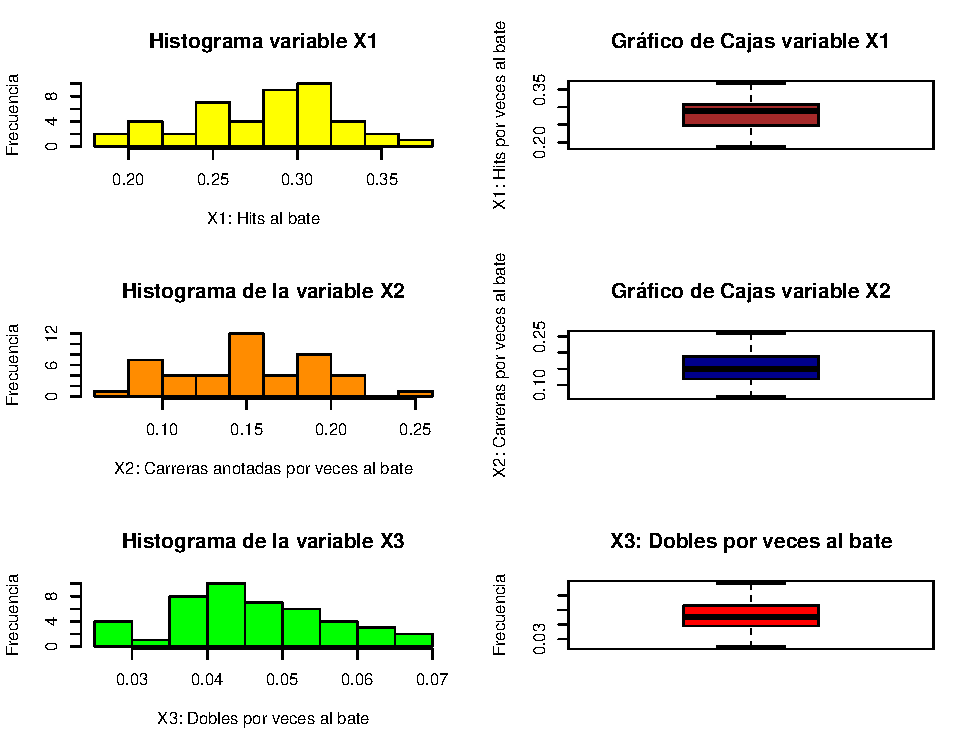
\includegraphics{C03322-InformeFinal-Cordero-Gavazut-Riera_files/figure-latex/boxplots-1.pdf}
  	\caption{\label{fig:boxplots}Histograma y gráfico de cajas para las variables}
  \end{figure}
 
 \newpage
 
 \hypertarget{anexo}{%
 \subsection{Anexo}\label{anexo}}
 \begin{figure}
 \centering
 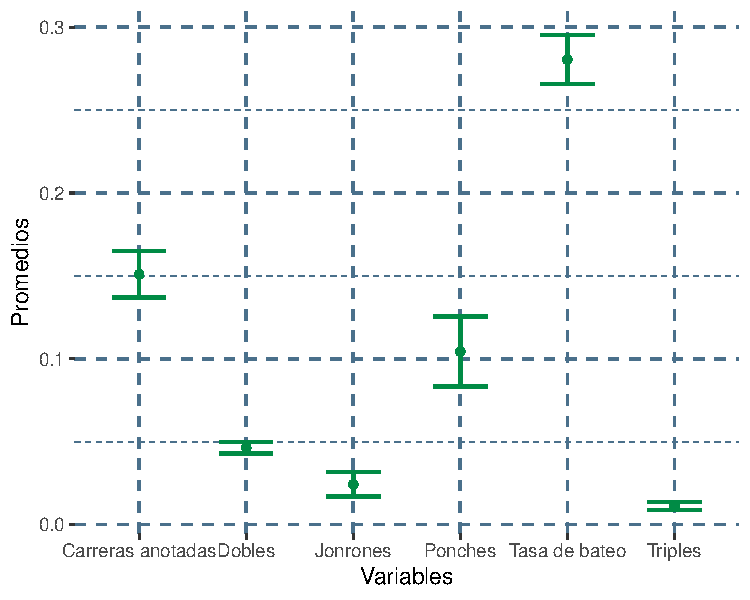
\includegraphics{C03322-InformeFinal-Cordero-Gavazut-Riera_files/figure-latex/interconf-1.pdf}
 \caption{\label{fig:interconf}Rpresentación gráfica de los intervalos de confianza para las medias}
 \end{figure}

 Codigos utilizados en este informe:

 \textbf{Obtener los estadísticos}

\begin{Shaded}
\begin{Highlighting}[]
\CommentTok{\# Función para obtener un resumen estadístico completo de cada variable}
\NormalTok{estadisticos}\OtherTok{\textless{}{-}} \ControlFlowTok{function}\NormalTok{(variables)\{}
  \CommentTok{\# Inicializamos las variables}
\NormalTok{  k}\OtherTok{\textless{}{-}} \FunctionTok{length}\NormalTok{(variables)}
  \CommentTok{\# Minimo }
\NormalTok{  minimo }\OtherTok{\textless{}{-}} \FunctionTok{rep}\NormalTok{(}\DecValTok{0}\NormalTok{,k)}
  \CommentTok{\# Media}
\NormalTok{  media }\OtherTok{\textless{}{-}} \FunctionTok{rep}\NormalTok{(}\DecValTok{0}\NormalTok{,k)}
  \CommentTok{\# Mediana}
\NormalTok{  mediana}\OtherTok{\textless{}{-}} \FunctionTok{rep}\NormalTok{(}\DecValTok{0}\NormalTok{,k)}
  \CommentTok{\# Cuartile 1: 25\%}
\NormalTok{  q1 }\OtherTok{\textless{}{-}}\FunctionTok{rep}\NormalTok{(}\DecValTok{0}\NormalTok{,k)}
  \CommentTok{\# Cuartile 3: 75\%}
\NormalTok{  q3 }\OtherTok{\textless{}{-}} \FunctionTok{rep}\NormalTok{(}\DecValTok{0}\NormalTok{,k)}
  \CommentTok{\# Maximo }
\NormalTok{  maximo }\OtherTok{\textless{}{-}} \FunctionTok{rep}\NormalTok{(}\DecValTok{0}\NormalTok{,k)}
  \CommentTok{\# Rango Intercuartile }
\NormalTok{  ric }\OtherTok{\textless{}{-}} \FunctionTok{rep}\NormalTok{(}\DecValTok{0}\NormalTok{,k)}
  \CommentTok{\# Varianza }
\NormalTok{  varianza }\OtherTok{\textless{}{-}} \FunctionTok{rep}\NormalTok{(}\DecValTok{0}\NormalTok{,k)}
  \CommentTok{\# Desviación estándar}
\NormalTok{  stad }\OtherTok{\textless{}{-}}\FunctionTok{rep}\NormalTok{(}\DecValTok{0}\NormalTok{,k)}
  \CommentTok{\# Coeficiente de variación}
\NormalTok{  coef\_var }\OtherTok{\textless{}{-}}  \FunctionTok{rep}\NormalTok{(}\DecValTok{0}\NormalTok{,k)}
  
  \ControlFlowTok{for}\NormalTok{(i }\ControlFlowTok{in} \DecValTok{1}\SpecialCharTok{:}\NormalTok{k)\{}
    \CommentTok{\# Minimo }
\NormalTok{    minimo[i] }\OtherTok{\textless{}{-}} \FunctionTok{min}\NormalTok{(variables[,i])}
    \CommentTok{\# Media}
\NormalTok{    media[i] }\OtherTok{\textless{}{-}} \FunctionTok{mean}\NormalTok{(variables[,i])}
    \CommentTok{\# Mediana}
\NormalTok{    mediana[i]}\OtherTok{\textless{}{-}} \FunctionTok{median}\NormalTok{(variables[,i])}
    \CommentTok{\# Cuartile 1: 25\%}
\NormalTok{    q1[i] }\OtherTok{\textless{}{-}} \FunctionTok{quantile}\NormalTok{(variables[,i],}\FloatTok{0.25}\NormalTok{)}
    \CommentTok{\# Cuartile 3: 75\%}
\NormalTok{    q3[i] }\OtherTok{\textless{}{-}} \FunctionTok{quantile}\NormalTok{(variables[,i],}\FloatTok{0.75}\NormalTok{)}
    \CommentTok{\# Maximo }
\NormalTok{    maximo[i] }\OtherTok{\textless{}{-}} \FunctionTok{max}\NormalTok{(variables[,i])}
    \CommentTok{\# Rango Intercuartile }
\NormalTok{    ric[i] }\OtherTok{\textless{}{-}} \FunctionTok{IQR}\NormalTok{(variables[,i])}
    \CommentTok{\# Varianza }
\NormalTok{    varianza[i] }\OtherTok{\textless{}{-}} \FunctionTok{var}\NormalTok{(variables[,i])}
    \CommentTok{\# Desviación estándar}
\NormalTok{    stad[i] }\OtherTok{\textless{}{-}} \FunctionTok{sd}\NormalTok{(variables[,i])}
    \CommentTok{\# Coeficiente de variación}
\NormalTok{    coef\_var }\OtherTok{\textless{}{-}}\NormalTok{  stad}\SpecialCharTok{/}\NormalTok{media }
\NormalTok{  \}}
  
  \CommentTok{\# Unimos los valores obtenidos}
\NormalTok{  estadisticos }\OtherTok{\textless{}{-}} \FunctionTok{cbind}\NormalTok{(}\FunctionTok{round}\NormalTok{(minimo, }\AttributeTok{digits=}\DecValTok{4}\NormalTok{),}\FunctionTok{round}\NormalTok{(q1, }\AttributeTok{digits =} \DecValTok{4}\NormalTok{),}
                        \FunctionTok{round}\NormalTok{(media, }\AttributeTok{digits=}\DecValTok{4}\NormalTok{), }\FunctionTok{round}\NormalTok{(mediana,}\AttributeTok{digits=}\DecValTok{4}\NormalTok{),}
                        \FunctionTok{round}\NormalTok{(q3, }\AttributeTok{digits=}\DecValTok{4}\NormalTok{), }\FunctionTok{round}\NormalTok{(maximo, }\AttributeTok{digits=}\DecValTok{4}\NormalTok{),}
                        \FunctionTok{round}\NormalTok{(ric, }\AttributeTok{digits=}\DecValTok{4}\NormalTok{),}\FunctionTok{round}\NormalTok{(varianza, }\AttributeTok{digits=}\DecValTok{4}\NormalTok{), }
                        \FunctionTok{round}\NormalTok{(stad, }\AttributeTok{digits=}\DecValTok{4}\NormalTok{), }\FunctionTok{round}\NormalTok{(coef\_var, }\AttributeTok{digits=}\DecValTok{4}\NormalTok{))}
  \CommentTok{\# Definimos los nombres de las columnas y filas}
  \FunctionTok{rownames}\NormalTok{(estadisticos) }\OtherTok{\textless{}{-}} \FunctionTok{c}\NormalTok{(}\StringTok{"X1"}\NormalTok{, }\StringTok{"X2"}\NormalTok{, }\StringTok{"X3"}\NormalTok{, }\StringTok{"X4"}\NormalTok{, }\StringTok{"X5"}\NormalTok{, }\StringTok{"X6"}\NormalTok{) }
  \FunctionTok{colnames}\NormalTok{(estadisticos) }\OtherTok{\textless{}{-}} \FunctionTok{c}\NormalTok{(}\StringTok{"Minimo"}\NormalTok{, }\StringTok{"25\%"}\NormalTok{, }\StringTok{"Media"}\NormalTok{, }\StringTok{"Mediana / 50"}\NormalTok{ ,}
                              \StringTok{"75\%"}\NormalTok{, }\StringTok{"Máximo"}\NormalTok{, }\StringTok{"RIC"}\NormalTok{,}\StringTok{"Varianza"}\NormalTok{, }
                              \StringTok{"Desv. Estándar"}\NormalTok{,}\StringTok{"Coef. Variación"}\NormalTok{)}
  \CommentTok{\# Mostramos el arreglo}
  \FunctionTok{return}\NormalTok{(estadisticos)}
  
\NormalTok{\}}
\NormalTok{variables }\OtherTok{\textless{}{-}}\FunctionTok{as.data.frame}\NormalTok{(Baseball)}
\end{Highlighting}
\end{Shaded}

 \textbf{Obtener las gráficas}

\begin{Shaded}
\begin{Highlighting}[]
\CommentTok{\# Se crea una matriz que defina el layout de las graficas }
\FunctionTok{par}\NormalTok{(}\AttributeTok{mfrow=}\FunctionTok{c}\NormalTok{(}\DecValTok{6}\NormalTok{,}\DecValTok{2}\NormalTok{), }\AttributeTok{mai=}\FunctionTok{c}\NormalTok{(}\FloatTok{0.4}\NormalTok{,}\FloatTok{0.4}\NormalTok{,}\FloatTok{0.4}\NormalTok{,}\FloatTok{0.4}\NormalTok{), }\AttributeTok{mgp=}\FunctionTok{c}\NormalTok{(}\FloatTok{1.8}\NormalTok{,}\FloatTok{0.6}\NormalTok{,}\FloatTok{0.3}\NormalTok{))}

\FunctionTok{hist}\NormalTok{(X1, }\AttributeTok{main =} \StringTok{"Histograma: Tasa de hits"}\NormalTok{, }\AttributeTok{ylab =} \StringTok{"Frecuencia"}\NormalTok{,}
     \AttributeTok{xlab =} \StringTok{"X1: Hits al bate"}\NormalTok{, }\AttributeTok{col=}\StringTok{"skyblue4"}\NormalTok{)}
\FunctionTok{boxplot}\NormalTok{(X1, }\AttributeTok{main =} \StringTok{"Gráfico de Cajas: Tasa de hits"}\NormalTok{, }\AttributeTok{xlab=}\StringTok{"Frecuencia"}\NormalTok{, }
        \AttributeTok{col=}\StringTok{"springgreen4"}\NormalTok{, }\AttributeTok{horizontal =}\NormalTok{ T)}

\FunctionTok{hist}\NormalTok{(X2, }\AttributeTok{main =} \StringTok{"Histograma: Tasa carreras anotadas"}\NormalTok{, }\AttributeTok{ylab =} \StringTok{"Frecuencia"}\NormalTok{, }
     \AttributeTok{xlab =} \StringTok{"X2: Tasa de carreras anotadas"}\NormalTok{, }\AttributeTok{col=}\StringTok{"skyblue3"}\NormalTok{)}
\FunctionTok{boxplot}\NormalTok{(X2, }\AttributeTok{main =} \StringTok{"Gráfico de Cajas: Tasa carreras anotadas"}\NormalTok{, }\AttributeTok{xlab=}\StringTok{"Frecuencia"}\NormalTok{, }
        \AttributeTok{col=}\StringTok{"springgreen3"}\NormalTok{, }\AttributeTok{horizontal =}\NormalTok{ T)}

\FunctionTok{hist}\NormalTok{(X3, }\AttributeTok{main =} \StringTok{"Histograma: Tasa de dobles"}\NormalTok{, }\AttributeTok{ylab=} \StringTok{"Frecuencia"}\NormalTok{, }
     \AttributeTok{xlab=} \StringTok{"X3: Dobles por veces al bate"}\NormalTok{, }\AttributeTok{col=}\StringTok{"skyblue2"}\NormalTok{)}
\FunctionTok{boxplot}\NormalTok{(X3, }\AttributeTok{main =} \StringTok{"Gráfico de Cajas: Tasa de dobles"}\NormalTok{, }\AttributeTok{xlab =} \StringTok{"Frecuencia"}\NormalTok{, }
        \AttributeTok{col =} \StringTok{"springgreen2"}\NormalTok{, }\AttributeTok{horizontal =}\NormalTok{ T)}

\FunctionTok{hist}\NormalTok{(X4, }\AttributeTok{main=}\StringTok{"Histograma: Tasa de triples"}\NormalTok{, }\AttributeTok{ylab =}\StringTok{"Frecuencia"}\NormalTok{, }
     \AttributeTok{xlab=}\StringTok{"X4: Triples por veces al bate"}\NormalTok{, }\AttributeTok{col =}\StringTok{"skyblue1"}\NormalTok{)}
\FunctionTok{boxplot}\NormalTok{(X4, }\AttributeTok{main =} \StringTok{"Gráfico de Cajas: Tasa de triples"}\NormalTok{, }\AttributeTok{xlab =} \StringTok{"Frecuencia"}\NormalTok{, }
        \AttributeTok{col =} \StringTok{"springgreen1"}\NormalTok{, }\AttributeTok{horizontal =}\NormalTok{ T)}

\FunctionTok{hist}\NormalTok{(X5, }\AttributeTok{main =} \StringTok{"Histograma: Tasa de jonrones"}\NormalTok{, }\AttributeTok{ylab =} \StringTok{"Frecuencia"}\NormalTok{, }
     \AttributeTok{xlab =} \StringTok{"X5: Jonrones por veces al bate"}\NormalTok{, }\AttributeTok{col=}\StringTok{"skyblue"}\NormalTok{)}
\FunctionTok{boxplot}\NormalTok{(X5, }\AttributeTok{main =} \StringTok{"Gráfico de Cajas: Tasa de jonrones"}\NormalTok{,}\AttributeTok{xlab=}\StringTok{"Frecuencia"}\NormalTok{, }
        \AttributeTok{col=}\StringTok{"springgreen"}\NormalTok{, }\AttributeTok{horizontal =}\NormalTok{ T)}

\FunctionTok{hist}\NormalTok{(X6, }\AttributeTok{main =} \StringTok{"Histograma: Tasa de ponches"}\NormalTok{, }\AttributeTok{ylab =} \StringTok{"Frecuencia"}\NormalTok{, }
     \AttributeTok{xlab =} \StringTok{"X6: Ponches por veces al bate"}\NormalTok{, }\AttributeTok{col=}\StringTok{"skyblue"}\NormalTok{)}
\FunctionTok{boxplot}\NormalTok{(X6, }\AttributeTok{main =} \StringTok{"Gráfico de Cajas: Tasa de ponches"}\NormalTok{, }\AttributeTok{xlab=}\StringTok{"Frecuencia"}\NormalTok{, }
        \AttributeTok{col=}\StringTok{"springgreen"}\NormalTok{, }\AttributeTok{horizontal =}\NormalTok{ T)}
\end{Highlighting}
\end{Shaded}

 \textbf{Intervalo de confianza para la media de las variables}

 \textbf{Prueba de hipotesis para la tasa de bateo }

\begin{Shaded}
\begin{Highlighting}[]
\FunctionTok{t.test}\NormalTok{(X1, }\AttributeTok{alternative =} \StringTok{"greater"}\NormalTok{, }\AttributeTok{mu=}\FloatTok{0.3}\NormalTok{, }\AttributeTok{conf.level =} \FloatTok{0.95}\NormalTok{)}
\end{Highlighting}
\end{Shaded}

\begin{verbatim}
## 
##  One Sample t-test
## 
## data:  X1
## t = -2.9779, df = 44, p-value = 0.9976
## alternative hypothesis: true mean is greater than 0.3
## 95 percent confidence interval:
##  0.2694453       Inf
## sample estimates:
## mean of x 
## 0.2804667
\end{verbatim}

 \textbf{Prueba de hipotesis para la tasa de jonrones y ponches}

\begin{Shaded}
\begin{Highlighting}[]
\FunctionTok{t.test}\NormalTok{(jonrones, ponches, }\AttributeTok{alternative=}\StringTok{\textquotesingle{}two.sided\textquotesingle{}}\NormalTok{)}
\end{Highlighting}
\end{Shaded}

\begin{verbatim}
## 
##  Welch Two Sample t-test
## 
## data:  jonrones and ponches
## t = -7.0502, df = 42.827, p-value = 1.112e-08
## alternative hypothesis: true difference in means is not equal to 0
## 95 percent confidence interval:
##  -0.10681617 -0.05929494
## sample estimates:
##  mean of x  mean of y 
## 0.02544444 0.10850000
\end{verbatim}

 \textbf{Prueba de bondad de ajuste}

\begin{Shaded}
\begin{Highlighting}[]
\CommentTok{\# Tamaño de los fi}
\NormalTok{(k}\OtherTok{\textless{}{-}} \FunctionTok{length}\NormalTok{(fi))}
\end{Highlighting}
\end{Shaded}

\begin{verbatim}
## [1] 5
\end{verbatim}

\begin{Shaded}
\begin{Highlighting}[]
\CommentTok{\# Numero total de datos }
\NormalTok{n}\OtherTok{\textless{}{-}} \FunctionTok{sum}\NormalTok{(fi)}
\CommentTok{\# Puntos medios de los intervalos}
\NormalTok{(mi}\OtherTok{\textless{}{-}}\FunctionTok{c}\NormalTok{(}\FloatTok{0.18}\SpecialCharTok{+}\NormalTok{(}\FloatTok{0.24{-}0.18}\NormalTok{)}\SpecialCharTok{/}\DecValTok{2}\NormalTok{,}\FloatTok{0.24}\SpecialCharTok{+}\NormalTok{(}\FloatTok{0.28{-}0.24}\NormalTok{)}\SpecialCharTok{/}\DecValTok{2}\NormalTok{,}\FloatTok{0.28}\SpecialCharTok{+}\NormalTok{(}\FloatTok{0.30{-}0.28}\NormalTok{)}\SpecialCharTok{/}\DecValTok{2}\NormalTok{,}
       \FloatTok{0.30}\SpecialCharTok{+}\NormalTok{(}\FloatTok{0.32{-}0.30}\NormalTok{)}\SpecialCharTok{/}\DecValTok{2}\NormalTok{, }\FloatTok{0.32}\SpecialCharTok{+}\NormalTok{(}\FloatTok{0.38{-}0.32}\NormalTok{)}\SpecialCharTok{/}\DecValTok{2}\NormalTok{))}
\end{Highlighting}
\end{Shaded}

\begin{verbatim}
## [1] 0.21 0.26 0.29 0.31 0.35
\end{verbatim}

\begin{Shaded}
\begin{Highlighting}[]
\CommentTok{\# Media de los datos}
\NormalTok{(xbarra}\OtherTok{\textless{}{-}}\FunctionTok{sum}\NormalTok{(fi}\SpecialCharTok{*}\NormalTok{mi)}\SpecialCharTok{/}\NormalTok{n)}
\end{Highlighting}
\end{Shaded}

\begin{verbatim}
## [1] 0.2822222
\end{verbatim}

\begin{Shaded}
\begin{Highlighting}[]
\CommentTok{\# Vector con las medias}
\NormalTok{x\_barra}\OtherTok{\textless{}{-}}\FunctionTok{rep}\NormalTok{(xbarra,k)}

\CommentTok{\# Varianza }
\NormalTok{(S\_cuadrado}\OtherTok{\textless{}{-}}\FunctionTok{sum}\NormalTok{(fi}\SpecialCharTok{*}\NormalTok{(mi}\SpecialCharTok{{-}}\NormalTok{x\_barra)}\SpecialCharTok{\^{}}\NormalTok{\{}\DecValTok{2}\NormalTok{\})}\SpecialCharTok{/}\NormalTok{(n}\DecValTok{{-}1}\NormalTok{))}
\end{Highlighting}
\end{Shaded}

\begin{verbatim}
## [1] 0.001990404
\end{verbatim}

\begin{Shaded}
\begin{Highlighting}[]
\CommentTok{\# Desviación estandar}
\NormalTok{(S}\OtherTok{\textless{}{-}}\FunctionTok{sqrt}\NormalTok{(S\_cuadrado))}
\end{Highlighting}
\end{Shaded}

\begin{verbatim}
## [1] 0.04461394
\end{verbatim}

\begin{Shaded}
\begin{Highlighting}[]
\CommentTok{\#calculemos los pi}
\CommentTok{\# P(Z\textless{}0.24)}
\NormalTok{(p1}\OtherTok{\textless{}{-}}\FunctionTok{pnorm}\NormalTok{(}\FloatTok{0.24}\NormalTok{,}\AttributeTok{mean=}\NormalTok{ xbarra,}\AttributeTok{sd=}\NormalTok{S))}
\end{Highlighting}
\end{Shaded}

\begin{verbatim}
## [1] 0.1719747
\end{verbatim}

\begin{Shaded}
\begin{Highlighting}[]
\CommentTok{\# P(0.24 \textless{} Z \textless{} 0.28) }
\NormalTok{(p2}\OtherTok{\textless{}{-}}\FunctionTok{pnorm}\NormalTok{(}\FloatTok{0.28}\NormalTok{,}\AttributeTok{mean=}\NormalTok{ xbarra,}\AttributeTok{sd=}\NormalTok{S)}\SpecialCharTok{{-}}\FunctionTok{pnorm}\NormalTok{(}\FloatTok{0.24}\NormalTok{,}\AttributeTok{mean=}\NormalTok{ xbarra,}\AttributeTok{sd=}\NormalTok{S))}
\end{Highlighting}
\end{Shaded}

\begin{verbatim}
## [1] 0.3081622
\end{verbatim}

\begin{Shaded}
\begin{Highlighting}[]
\NormalTok{(p3}\OtherTok{\textless{}{-}}\FunctionTok{pnorm}\NormalTok{(}\FloatTok{0.30}\NormalTok{,}\AttributeTok{mean=}\NormalTok{ xbarra,}\AttributeTok{sd=}\NormalTok{S)}\SpecialCharTok{{-}}\FunctionTok{pnorm}\NormalTok{(}\FloatTok{0.28}\NormalTok{,}\AttributeTok{mean=}\NormalTok{ xbarra,}\AttributeTok{sd=}\NormalTok{S))}
\end{Highlighting}
\end{Shaded}

\begin{verbatim}
## [1] 0.174725
\end{verbatim}

\begin{Shaded}
\begin{Highlighting}[]
\NormalTok{(p4}\OtherTok{\textless{}{-}}\FunctionTok{pnorm}\NormalTok{(}\FloatTok{0.32}\NormalTok{,}\AttributeTok{mean=}\NormalTok{ xbarra,}\AttributeTok{sd=}\NormalTok{S)}\SpecialCharTok{{-}}\FunctionTok{pnorm}\NormalTok{(}\FloatTok{0.30}\NormalTok{,}\AttributeTok{mean=}\NormalTok{ xbarra,}\AttributeTok{sd=}\NormalTok{S))}
\end{Highlighting}
\end{Shaded}

\begin{verbatim}
## [1] 0.1465766
\end{verbatim}

\begin{Shaded}
\begin{Highlighting}[]
\NormalTok{(p5}\OtherTok{\textless{}{-}}\FunctionTok{pnorm}\NormalTok{(}\FloatTok{0.32}\NormalTok{,}\AttributeTok{mean=}\NormalTok{ xbarra,}\AttributeTok{sd=}\NormalTok{S, }\AttributeTok{lower.tail =}\NormalTok{ F))}
\end{Highlighting}
\end{Shaded}

\begin{verbatim}
## [1] 0.1985615
\end{verbatim}

\begin{Shaded}
\begin{Highlighting}[]
\CommentTok{\# Vector con las probabilidades}
\NormalTok{(pi}\OtherTok{\textless{}{-}}\FunctionTok{c}\NormalTok{(p1,p2,p3,p4,p5))}
\end{Highlighting}
\end{Shaded}

\begin{verbatim}
## [1] 0.1719747 0.3081622 0.1747250 0.1465766 0.1985615
\end{verbatim}

\begin{Shaded}
\begin{Highlighting}[]
\CommentTok{\# Suma de las probabilidades}
\NormalTok{(}\FunctionTok{sum}\NormalTok{(pi))}
\end{Highlighting}
\end{Shaded}

\begin{verbatim}
## [1] 1
\end{verbatim}

\begin{Shaded}
\begin{Highlighting}[]
\CommentTok{\# Estadistico}
\NormalTok{(t}\OtherTok{\textless{}{-}}\FunctionTok{sum}\NormalTok{(((fi}\SpecialCharTok{{-}}\NormalTok{n}\SpecialCharTok{*}\NormalTok{pi)}\SpecialCharTok{\^{}}\NormalTok{\{}\DecValTok{2}\NormalTok{\})}\SpecialCharTok{/}\NormalTok{(n}\SpecialCharTok{*}\NormalTok{pi)))}
\end{Highlighting}
\end{Shaded}

\begin{verbatim}
## [1] 2.942129
\end{verbatim}

\begin{Shaded}
\begin{Highlighting}[]
\CommentTok{\# p{-}valor}
\NormalTok{(p\_Valor}\OtherTok{\textless{}{-}} \DecValTok{1}\SpecialCharTok{{-}}\FunctionTok{pchisq}\NormalTok{(t,k}\DecValTok{{-}1{-}2}\NormalTok{))}
\end{Highlighting}
\end{Shaded}

\begin{verbatim}
## [1] 0.2296808
\end{verbatim}

 \textbf{Matriz de correlación}

\begin{Shaded}
\begin{Highlighting}[]
\DocumentationTok{\#\# Codigo de R{-}coder https://r{-}coder.com/grafico{-}correlacion{-}r/}
\NormalTok{panel.cor }\OtherTok{\textless{}{-}} \ControlFlowTok{function}\NormalTok{(x, y, }\AttributeTok{digits =} \DecValTok{2}\NormalTok{, }\AttributeTok{prefix =} \StringTok{""}\NormalTok{, cex.cor, ...) \{}
\NormalTok{    usr }\OtherTok{\textless{}{-}} \FunctionTok{par}\NormalTok{(}\StringTok{"usr"}\NormalTok{)}
    \FunctionTok{on.exit}\NormalTok{(}\FunctionTok{par}\NormalTok{(usr))}
    \FunctionTok{par}\NormalTok{(}\AttributeTok{usr =} \FunctionTok{c}\NormalTok{(}\DecValTok{0}\NormalTok{, }\DecValTok{1}\NormalTok{, }\DecValTok{0}\NormalTok{, }\DecValTok{1}\NormalTok{))}
\NormalTok{    Cor }\OtherTok{\textless{}{-}} \FunctionTok{cor}\NormalTok{(x, y) }\CommentTok{\# Elimina la función abs si lo prefieres}
\NormalTok{    txt }\OtherTok{\textless{}{-}} \FunctionTok{paste0}\NormalTok{(prefix, }\FunctionTok{format}\NormalTok{(}\FunctionTok{c}\NormalTok{(Cor, }\FloatTok{0.123456789}\NormalTok{), }\AttributeTok{digits =}\NormalTok{ digits)[}\DecValTok{1}\NormalTok{])}
    \ControlFlowTok{if}\NormalTok{(}\FunctionTok{missing}\NormalTok{(cex.cor)) \{}
\NormalTok{        cex.cor }\OtherTok{\textless{}{-}} \FloatTok{0.4} \SpecialCharTok{/} \FunctionTok{strwidth}\NormalTok{(txt)}
\NormalTok{    \}}
    \FunctionTok{text}\NormalTok{(}\FloatTok{0.5}\NormalTok{, }\FloatTok{0.5}\NormalTok{, txt,}
         \AttributeTok{cex =} \DecValTok{1} \SpecialCharTok{+}\NormalTok{ cex.cor) }\CommentTok{\# Escala el texto al nivel de correlación}
\NormalTok{\}}
\CommentTok{\# Dibujamos la matriz de correlación}
\FunctionTok{pairs}\NormalTok{(Baseball,}
      \AttributeTok{label=}\FunctionTok{c}\NormalTok{(}\StringTok{"Bateo"}\NormalTok{,}\StringTok{"Carreras"}\NormalTok{,}\StringTok{"Dobles"}\NormalTok{, }\StringTok{"Triples"}\NormalTok{, }\StringTok{"Jonrones"}\NormalTok{, }\StringTok{"Ponches"}\NormalTok{),}
      \AttributeTok{upper.panel =}\NormalTok{ panel.cor,    }\CommentTok{\# Panel de correlación}
      \AttributeTok{col =} \FunctionTok{c}\NormalTok{(}\StringTok{"springgreen3"}\NormalTok{),  }\CommentTok{\# Colores de los puntos}
      \AttributeTok{bg =} \FunctionTok{c}\NormalTok{(}\StringTok{"springgreen3"}\NormalTok{),   }\CommentTok{\# Colores de los puntos}
      \AttributeTok{pch =} \DecValTok{21}\NormalTok{,                   }\CommentTok{\# Símbolo pch}
      \AttributeTok{main =} \StringTok{"Matriz de Correlación de las variables"}\NormalTok{,  }\CommentTok{\# Titulo}
      \AttributeTok{cex.labels =} \ConstantTok{NULL}\NormalTok{,        }\CommentTok{\# Tamaño del texto de la diagonal}
      \AttributeTok{font.labels =} \DecValTok{1}          \CommentTok{\# Estilo de fuente del texto de la diagonal}
\NormalTok{)}
\end{Highlighting}
\end{Shaded}

 \textbf{Modelo lineal}

\begin{Shaded}
\begin{Highlighting}[]
\NormalTok{n }\OtherTok{\textless{}{-}} \DecValTok{36}
\FunctionTok{set.seed}\NormalTok{(}\DecValTok{777}\NormalTok{)}

\NormalTok{elegidos }\OtherTok{\textless{}{-}} \FunctionTok{sort}\NormalTok{(}\FunctionTok{sample}\NormalTok{(}\FunctionTok{seq\_len}\NormalTok{(}\FunctionTok{nrow}\NormalTok{(Baseball)),}\AttributeTok{size =}\NormalTok{ n))}
\NormalTok{Baseball\_80 }\OtherTok{\textless{}{-}}\NormalTok{ Baseball[elegidos, ]}
\NormalTok{Baseball\_20 }\OtherTok{\textless{}{-}}\NormalTok{ Baseball[}\SpecialCharTok{{-}}\NormalTok{elegidos, ]}
\end{Highlighting}
\end{Shaded}

 1 era prueba

\begin{Shaded}
\begin{Highlighting}[]
\NormalTok{tasa\_de\_bateo }\OtherTok{\textless{}{-}}\NormalTok{ Baseball\_80}\SpecialCharTok{$}\NormalTok{X1}
\NormalTok{carreras }\OtherTok{\textless{}{-}}\NormalTok{ Baseball\_80}\SpecialCharTok{$}\NormalTok{X2}
\NormalTok{dobles }\OtherTok{\textless{}{-}}\NormalTok{ Baseball\_80}\SpecialCharTok{$}\NormalTok{X3}
\NormalTok{triples }\OtherTok{\textless{}{-}}\NormalTok{ Baseball\_80}\SpecialCharTok{$}\NormalTok{X4}
\NormalTok{jonrones }\OtherTok{\textless{}{-}}\NormalTok{ Baseball\_80}\SpecialCharTok{$}\NormalTok{X5}
\NormalTok{ponches }\OtherTok{\textless{}{-}}\NormalTok{ Baseball\_80}\SpecialCharTok{$}\NormalTok{X6}

\NormalTok{m1 }\OtherTok{\textless{}{-}} \FunctionTok{lm}\NormalTok{(tasa\_de\_bateo }\SpecialCharTok{\textasciitilde{}}\NormalTok{ carreras }\SpecialCharTok{+}\NormalTok{ dobles }\SpecialCharTok{+}\NormalTok{ triples }\SpecialCharTok{+}\NormalTok{ jonrones }\SpecialCharTok{+}\NormalTok{ ponches)}
\FunctionTok{summary}\NormalTok{(m1)}
\end{Highlighting}
\end{Shaded}

\begin{verbatim}
## 
## Call:
## lm(formula = tasa_de_bateo ~ carreras + dobles + triples + jonrones + 
##     ponches)
## 
## Residuals:
##       Min        1Q    Median        3Q       Max 
## -0.038609 -0.011625  0.001590  0.008057  0.034985 
## 
## Coefficients:
##             Estimate Std. Error t value Pr(>|t|)    
## (Intercept)  0.18250    0.01816  10.049 4.08e-11 ***
## carreras     0.35996    0.11455   3.142  0.00376 ** 
## dobles       1.22453    0.37152   3.296  0.00253 ** 
## triples      0.55428    0.62532   0.886  0.38245    
## jonrones     0.39297    0.18458   2.129  0.04158 *  
## ponches     -0.28815    0.05097  -5.653 3.69e-06 ***
## ---
## Signif. codes:  0 '***' 0.001 '**' 0.01 '*' 0.05 '.' 0.1 ' ' 1
## 
## Residual standard error: 0.01641 on 30 degrees of freedom
## Multiple R-squared:  0.8879, Adjusted R-squared:  0.8692 
## F-statistic: 47.53 on 5 and 30 DF,  p-value: 2.308e-13
\end{verbatim}

 2da prueba

\begin{Shaded}
\begin{Highlighting}[]
\NormalTok{m2 }\OtherTok{\textless{}{-}} \FunctionTok{lm}\NormalTok{(tasa\_de\_bateo }\SpecialCharTok{\textasciitilde{}}\NormalTok{ carreras }\SpecialCharTok{+}\NormalTok{ dobles }\SpecialCharTok{+}\NormalTok{ jonrones}\SpecialCharTok{+}\NormalTok{ ponches)}
\FunctionTok{summary}\NormalTok{(m2)}
\end{Highlighting}
\end{Shaded}

\begin{verbatim}
## 
## Call:
## lm(formula = tasa_de_bateo ~ carreras + dobles + jonrones + ponches)
## 
## Residuals:
##       Min        1Q    Median        3Q       Max 
## -0.035060 -0.012486  0.001372  0.007376  0.037906 
## 
## Coefficients:
##             Estimate Std. Error t value Pr(>|t|)    
## (Intercept)  0.17715    0.01707  10.379 1.31e-11 ***
## carreras     0.40656    0.10142   4.009 0.000357 ***
## dobles       1.36860    0.33292   4.111 0.000268 ***
## jonrones     0.32041    0.16486   1.944 0.061079 .  
## ponches     -0.29278    0.05053  -5.794 2.21e-06 ***
## ---
## Signif. codes:  0 '***' 0.001 '**' 0.01 '*' 0.05 '.' 0.1 ' ' 1
## 
## Residual standard error: 0.01635 on 31 degrees of freedom
## Multiple R-squared:  0.885,  Adjusted R-squared:  0.8701 
## F-statistic: 59.63 on 4 and 31 DF,  p-value: 4.07e-14
\end{verbatim}

 3ra prueba

\begin{Shaded}
\begin{Highlighting}[]
\NormalTok{m3 }\OtherTok{\textless{}{-}} \FunctionTok{lm}\NormalTok{(tasa\_de\_bateo }\SpecialCharTok{\textasciitilde{}}\NormalTok{ carreras }\SpecialCharTok{+}\NormalTok{ dobles }\SpecialCharTok{+}\NormalTok{ ponches)}
\FunctionTok{summary}\NormalTok{(m3)}
\end{Highlighting}
\end{Shaded}

\begin{verbatim}
## 
## Call:
## lm(formula = tasa_de_bateo ~ carreras + dobles + ponches)
## 
## Residuals:
##       Min        1Q    Median        3Q       Max 
## -0.035643 -0.009929 -0.001336  0.012005  0.036693 
## 
## Coefficients:
##             Estimate Std. Error t value Pr(>|t|)    
## (Intercept)  0.16301    0.01610  10.126 1.67e-11 ***
## carreras     0.51923    0.08676   5.985 1.13e-06 ***
## dobles       1.36501    0.34706   3.933 0.000423 ***
## ponches     -0.24507    0.04604  -5.323 7.77e-06 ***
## ---
## Signif. codes:  0 '***' 0.001 '**' 0.01 '*' 0.05 '.' 0.1 ' ' 1
## 
## Residual standard error: 0.01705 on 32 degrees of freedom
## Multiple R-squared:  0.871,  Adjusted R-squared:  0.8589 
## F-statistic:    72 on 3 and 32 DF,  p-value: 2.555e-14
\end{verbatim}

 Predicciones

\begin{Shaded}
\begin{Highlighting}[]
\NormalTok{predicciones }\OtherTok{\textless{}{-}} \FunctionTok{predict}\NormalTok{(m2,Baseball\_20, }\AttributeTok{interval=}\StringTok{"confidence"}\NormalTok{)}
\NormalTok{pre }\OtherTok{\textless{}{-}}\NormalTok{ predicciones[}\FunctionTok{c}\NormalTok{(}\DecValTok{1}\SpecialCharTok{:}\DecValTok{9}\NormalTok{)]}
\NormalTok{diferencia }\OtherTok{\textless{}{-}}\NormalTok{ Baseball\_20}\SpecialCharTok{$}\NormalTok{X1 }\SpecialCharTok{{-}}\NormalTok{ pre}
\NormalTok{tabla\_pre }\OtherTok{\textless{}{-}} \FunctionTok{cbind}\NormalTok{(Baseball\_20}\SpecialCharTok{$}\NormalTok{X1 , pre ,  diferencia) }
\FunctionTok{colnames}\NormalTok{(tabla\_pre) }\OtherTok{\textless{}{-}} \FunctionTok{c}\NormalTok{(}\StringTok{"Tasa de hits real "}\NormalTok{,}\StringTok{" Tasa de hits predicha "}\NormalTok{ , }\StringTok{" Diferencia "}\NormalTok{)}
\NormalTok{knitr}\SpecialCharTok{::}\FunctionTok{kable}\NormalTok{(tabla\_pre, }\AttributeTok{align =} \StringTok{"ccc"}\NormalTok{ , }\AttributeTok{caption =} \StringTok{"Hits reales vs Hits predichos"}\NormalTok{)}
\end{Highlighting}
\end{Shaded}

 \textbf{Modelo Anova}

\begin{Shaded}
\begin{Highlighting}[]
\NormalTok{grupo1}\OtherTok{\textless{}{-}} \FunctionTok{subset}\NormalTok{(Baseball, (X1}\SpecialCharTok{\textless{}}\FloatTok{0.200}\NormalTok{) )}
\NormalTok{grupo2}\OtherTok{\textless{}{-}} \FunctionTok{subset}\NormalTok{(Baseball, (X1 }\SpecialCharTok{\textgreater{}=} \FloatTok{0.200} \SpecialCharTok{\&}\NormalTok{ X1 }\SpecialCharTok{\textless{}=}\FloatTok{0.300}\NormalTok{))}
\NormalTok{grupo3}\OtherTok{\textless{}{-}} \FunctionTok{subset}\NormalTok{(Baseball, (X1}\SpecialCharTok{\textgreater{}=}\FloatTok{0.300}\NormalTok{))}

\NormalTok{media1}\OtherTok{\textless{}{-}} \FunctionTok{colMeans}\NormalTok{(grupo1[}\FunctionTok{sapply}\NormalTok{(grupo1, is.numeric)]) }
\NormalTok{media2}\OtherTok{\textless{}{-}} \FunctionTok{colMeans}\NormalTok{(grupo2[}\FunctionTok{sapply}\NormalTok{(grupo1, is.numeric)])}
\NormalTok{media3}\OtherTok{\textless{}{-}} \FunctionTok{colMeans}\NormalTok{(grupo3[}\FunctionTok{sapply}\NormalTok{(grupo1, is.numeric)])}

\NormalTok{medias }\OtherTok{\textless{}{-}} \FunctionTok{rbind}\NormalTok{(media1,media2,media3)}

\NormalTok{datos}\OtherTok{\textless{}{-}} \FunctionTok{c}\NormalTok{(medias[,}\DecValTok{1}\NormalTok{] , medias[,}\DecValTok{2}\NormalTok{], medias[,}\DecValTok{3}\NormalTok{],medias[,}\DecValTok{4}\NormalTok{],medias[,}\DecValTok{5}\NormalTok{],medias[,}\DecValTok{6}\NormalTok{])}

\NormalTok{variables }\OtherTok{\textless{}{-}} \FunctionTok{gl}\NormalTok{(}\DecValTok{6}\NormalTok{,}\DecValTok{3}\NormalTok{, }\AttributeTok{labels=}\FunctionTok{c}\NormalTok{(}\StringTok{"X1"}\NormalTok{,}\StringTok{"X2"}\NormalTok{,}\StringTok{"X3"}\NormalTok{,}\StringTok{"X4"}\NormalTok{,}\StringTok{"X5"}\NormalTok{,}\StringTok{"X6"}\NormalTok{))}
\NormalTok{grupos }\OtherTok{=} \FunctionTok{factor}\NormalTok{(}\FunctionTok{rep}\NormalTok{(}\DecValTok{1}\SpecialCharTok{:}\DecValTok{3}\NormalTok{,}\DecValTok{6}\NormalTok{), }\AttributeTok{labels=}\FunctionTok{c}\NormalTok{(}\StringTok{"Grupo1"}\NormalTok{,}\StringTok{"Grupo2"}\NormalTok{,}\StringTok{"Grupo3"}\NormalTok{))}
\FunctionTok{xtabs}\NormalTok{(datos}\SpecialCharTok{\textasciitilde{}}\NormalTok{grupos}\SpecialCharTok{+}\NormalTok{variables )}
\end{Highlighting}
\end{Shaded}

\begin{verbatim}
##         variables
## grupos           X1         X2         X3         X4         X5         X6
##   Grupo1 0.19350000 0.08200000 0.03650000 0.00700000 0.00650000 0.19650000
##   Grupo2 0.25804000 0.13276000 0.04144000 0.00872000 0.02228000 0.12048000
##   Grupo3 0.32127778 0.18372222 0.05427778 0.01533333 0.02900000 0.07166667
\end{verbatim}

\begin{Shaded}
\begin{Highlighting}[]
\FunctionTok{library}\NormalTok{(knitr)}
\FunctionTok{library}\NormalTok{(kableExtra)}

\FunctionTok{kable}\NormalTok{(}\FunctionTok{xtabs}\NormalTok{(datos}\SpecialCharTok{\textasciitilde{}}\NormalTok{grupos}\SpecialCharTok{+}\NormalTok{variables ),}
      \AttributeTok{caption =} \StringTok{"Tabla a dos factores para las medias de las variables"}\NormalTok{) }\SpecialCharTok{\%\textgreater{}\%}
  \FunctionTok{kable\_styling}\NormalTok{(}\AttributeTok{full\_width =}\NormalTok{ F)}
\end{Highlighting}
\end{Shaded}

\begin{Shaded}
\begin{Highlighting}[]
\CommentTok{\# Una variables }
\NormalTok{modelo.lineal }\OtherTok{=} \FunctionTok{lm}\NormalTok{(datos}\SpecialCharTok{\textasciitilde{}}\NormalTok{variables)}
\FunctionTok{anova}\NormalTok{(modelo.lineal)}
\end{Highlighting}
\end{Shaded}

\begin{verbatim}
## Analysis of Variance Table
## 
## Response: datos
##           Df   Sum Sq   Mean Sq F value    Pr(>F)    
## variables  5 0.133402 0.0266805  14.736 9.136e-05 ***
## Residuals 12 0.021727 0.0018105                      
## ---
## Signif. codes:  0 '***' 0.001 '**' 0.01 '*' 0.05 '.' 0.1 ' ' 1
\end{verbatim}

\begin{Shaded}
\begin{Highlighting}[]
\CommentTok{\# Dos variables}
\NormalTok{modelo.lineal2 }\OtherTok{=} \FunctionTok{lm}\NormalTok{(datos}\SpecialCharTok{\textasciitilde{}}\NormalTok{grupos}\SpecialCharTok{+}\NormalTok{variables)}
\NormalTok{prueba}\OtherTok{\textless{}{-}}\FunctionTok{anova}\NormalTok{(modelo.lineal2)}
\end{Highlighting}
\end{Shaded}

\begin{Shaded}
\begin{Highlighting}[]
\FunctionTok{kable}\NormalTok{(prueba,}\AttributeTok{caption =} \StringTok{"Tabla a dos factores para las medias de las variables"}\NormalTok{) }\SpecialCharTok{\%\textgreater{}\%}
  \FunctionTok{kable\_styling}\NormalTok{(}\AttributeTok{full\_width =}\NormalTok{ F)}
\end{Highlighting}
\end{Shaded}

	

\end{document}
